\documentclass[12pt,spanish,chapterprefix, numbers=noenddot]{book}
\usepackage{amsmath}
\usepackage{amsthm}
\usepackage{fontspec}
\usepackage[a4paper]{geometry}
\geometry{verbose,tmargin=2.5cm,bmargin=2.5cm,lmargin=2.5cm,rmargin=2.5cm,headheight=1cm,headsep=1cm,footskip=1cm}
\setlength{\parskip}{\medskipamount}
\setlength{\parindent}{0pt}
\usepackage{color}
\usepackage{babel}
\addto\shorthandsspanish{\spanishdeactivate{~<>}}

\usepackage{float}
\usepackage{makeidx}
\makeindex
\usepackage{graphicx}
\usepackage{nomencl}
% the following is useful when we have the old nomencl.sty package
\providecommand{\printnomenclature}{\printglossary}
\providecommand{\makenomenclature}{\makeglossary}
\makenomenclature
\usepackage[unicode=true,pdfusetitle,
    bookmarks=true,bookmarksnumbered=false,bookmarksopen=false,
    breaklinks=true,pdfborder={0 0 0},pdfborderstyle={},backref=false,colorlinks=true]
{hyperref}
\hypersetup{
    allcolors=blue}

\makeatletter

%%%%%%%%%%%%%%%%%%%%%%%%%%%%%% LyX specific LaTeX commands.
\newcommand{\noun}[1]{\textsc{#1}}
\providecommand\textquotedblplain{%
    \bgroup\addfontfeatures{Mapping=}\char34\egroup}
%% Because html converters don't know tabularnewline
\providecommand{\tabularnewline}{\\}
\floatstyle{ruled}
\newfloat{algorithm}{tbp}{loa}[chapter]
\providecommand{\algorithmname}{Algoritmo}
\floatname{algorithm}{\protect\algorithmname}

%%%%%%%%%%%%%%%%%%%%%%%%%%%%%% Textclass specific LaTeX commands.
\numberwithin{equation}{section}
\numberwithin{figure}{section}
\providecommand*{\code}[1]{\texttt{#1}}

%%%%%%%%%%%%%%%%%%%%%%%%%%%%%% User specified LaTeX commands.
%Para que las URLs de la bibliografía se pueda pinchar
\usepackage{url}

%Cabeceras y pies de página
\usepackage{fancyhdr}
\pagestyle{fancy}
\lhead[\rightmark]{}
\rhead[]{\leftmark}
\cfoot{\thepage}

%Para que los índices respeten los espacios de las nuemraciones
\usepackage[tocindentauto]{tocstyle}
\usetocstyle{standard}

%Para que ponga "Índice de Tablas" en vez de "Indice de Cuadros"
\addto\captionsspanish{
    \def\tablename{Tabla}
    \def\listtablename{\'Indice de tablas}
}

%Para que las páginas en blanco no tengan cabecera ni número de página
\makeatletter
\renewcommand*{\cleardoublepage}{\clearpage\if@twoside \ifodd\c@page\else
\hbox{}%
\thispagestyle{empty}%
\newpage%
\if@twocolumn\hbox{}\newpage\fi\fi\fi}
\makeatother



\usepackage{chngcntr}
\counterwithout{figure}{chapter}
\counterwithout{figure}{section}
\counterwithout{table}{chapter}
\counterwithout{algorithm}{chapter}

\AtBeginDocument{
    \def\labelitemii{\(\circ\)}
    \def\labelitemiii{\(\triangleright\)}
}

\makeatother

\usepackage{listings}
\lstset{basicstyle={\ttfamily},
    breaklines=true}
\usepackage[style=numeric,backref=true]{biblatex}
\def\eqdeclaration#1{, véase la ecuación\nobreakspace(#1)}
\def\pagedeclaration#1{, página\nobreakspace#1}
\def\nomname{Nomenclatura}
\renewcommand{\lstlistingname}{Listado de código}

\addbibresource{./refs.bib}
\begin{document}
    \frontmatter

    \begin{titlepage}

        \begin{center}
            
\includegraphics[width=8cm]{Figs/logoURJC}
            \par\end{center}

        \begin{center}
            Facultad de Ciencias Jurídicas y Sociales
            \par\end{center}

        \vspace{4cm}

        \begin{center}
        {\LARGE{}El futuro de la contabilidad descentralizada}{\LARGE\par}
            \par\end{center}

        \vspace{4cm}

        \begin{center}
        {\large{}Memoria del Trabajo Fin de Grado}{\large\par}
            \par\end{center}

        \begin{center}
        {\large{}en Administración y Dirección de Empresas}{\large\par}
            \par\end{center}

        \vspace{4cm}

        \begin{center}
        {\large{}Autor: }{\large\par}
            \par\end{center}

        \begin{center}
        {\large{}David García}{\large\par}
            \par\end{center}

        \begin{center}
        {\large{}Tutor: Almudena Macías}{\large\par}
            \par\end{center}

        \begin{center}
            Julio 2022
            \par\end{center}

    \end{titlepage}

    \chapter*{Agradecimientos}

    Quiero agradecer sus consejos a Cristina Rodríguez.

    Quiero agradecer su confianza a todos lo alumnos que me han permitido
    ser su tutor en su Trabajo Fin de Grado/Máster o Tesis. Gracias a
    ellos he conseguido la experiencia necesaria para escribir este documento.

    Quiero agradecer sus contribuciones a todos los desarrolladores de
    software libre que me han proporcionado herramientas para realizar
    este trabajo.

    Finalmente, quiero agradecer su paciencia a mi familia por el tiempo
    que les robo escribiendo estos manuales.

    \chapter*{Prólogo}

    Los alumnos de los Trabajos Fin de Titulación (TFT) suelen tener dudas
    a la hora de escribir la memoria de su trabajo. Las dudas de los alumnos
    abarcan la estructura que debe tener el documento, el contenido, la
    forma de escribir, la presentación, etc. Además, los alumnos suelen
    pedir un ejemplo a su tutor, pero normalmente el tutor no tiene documentos
    modélicos o no tiene permiso para facilitar documentos de otros alumnos.

    Por todo ello se decidió crear un documento con un triple objetivo:
    que explicase los detalles del proceso de creación de un TFT, que
    sirviese como ejemplo de memoria de TFT y que sirviese como plantilla.

    El presente documento es el resultado de un proceso de análisis de
    multitud de TFT en diferentes titulaciones. Este documento está dividido
    en varios capítulos. En todos los TFT analizados se ha encontrado
    un resumen, un índice, un capítulo inicial de introducción y un capítulo
    final de conclusiones, por ello este documento también sigue esta
    estructura. Además, este documento contiene capítulos que explican
    cómo son los índices de algunos TFT en distintas titulaciones, cómo
    usar el lenguaje para escribir un TFT, cómo usar el procesador de
    textos y cómo hacer una presentación oral efectiva.

    \tableofcontents{}

    \listoftables

    \listoffigures

    \listof{algorithm}{Algoritmos}

    \settowidth{\nomlabelwidth}{notepad}
    \printnomenclature{}

    \mainmatter

    \chapter{Introducción}

    La confección de la memoria es una parte fundamental del Trabajo Fin
    de Titulación\index{Trabajo Fin de Titulación} (\nomenclature{TFT}{Trabajo Fin de Grado}\index{TFT}TFT).
    Todos los textos y contenidos deben ser propios del estudiante, que
    debe encargarse de redactarlos, a partir del estudio, análisis, comparación
    y valoración de informaciones y datos procedentes de diversas fuentes
    ya sean directas e indirectas. Cualquier información no original debe
    ser citada convenientemente.

    Durante los siguientes capítulos se cubrirán tanto aspectos de contenido,
    como aspectos de estilo, formato y presentación.

    \section{Motivación}

    El objetivo de esta sección es el de presentar la motivación del trabajo
    que se ha desarrollado. Como es natural, los motivos pueden ser variados:
    resolver un problema no solucionado o parcialmente resuelto, mejorar
    alguna propuesta, estudiar un problema en profundidad, describir o
    interpretar con datos y en detalle un hecho, explicar la relación
    causa-efecto, comprobar la efectividad de un método, desarrollar un
    producto que cubra una necesidad social... Es una buena idea poner
    al lector en contexto. Se explica el problema, poniendo énfasis en
    la situación que hace necesario la realización del trabajo.

    Tras la creación del Espacio Europeo de Enseñanza Superior redactado
    en Bolonia en 1999 \cite{EEES}, es obligatorio que todo alumno de
    grado, máster y tesis realice un TFT. La escritura de la memoria de
    este trabajo suele ser una labor complicada ya que es la primera vez
    que el estudiante se enfrenta a redactar un documento extenso y con
    una estructura determinada. Habitualmente se sirven de otros trabajos
    de la misma titulación para tener un esquema de cómo realizar dicho
    documento. Esta tarea les exige leer dichas memorias y extraer la
    estructura y el contenido principal que deben trasladar a su documento.
    Al problema de redactar algo nuevo se une el desconocimiento de las
    herramientas informáticas que se deben usar para la escritura de la
    memoria y para la consulta de información.

    Los tutores (habitualmente los profesores) de los trabajos deben realizar
    una labor de guía y revisión de estos documentos, lo que frecuentemente
    les supone una inversión de tiempo y recursos que quitan a otras labores
    docentes e investigadoras. Además, esta tarea se repite cada vez que
    dirigen uno de estos trabajos lo que provoca que alguna vez se olviden
    de dar todas las orientaciones pertinentes a los estudiantes.

    Este documento pretende ser una guía que oriente al alumno en la confección
    de dicha memoria. El objetivo principal de este documento es la de
    dar pautas al alumno en cuanto a: estilo literario, formato del documento
    y uso de herramientas informáticas.

    Para terminar esta sección, se remarca que es una buena idea escribir
    la sección de motivación en las primeras fases del TFT, pues ayuda
    a enfocar su desarrollo. Normalmente, esta sección está fuertemente
    influenciada por el tutor (o director), ya que es el que generalmente
    plantea el problema. Es por ello que su supervisión es fundamental.
    Además, esta sección es una de las que más carga bibliográfica tienen.

    \section{Metodología}

    Una vez presentado el problema y el contexto en el que se desarrollará
    la posible solución, hay que hacer un estudio sobre las soluciones
    (parciales) que se han propuesto antes del desarrollo del TFT. Esto
    exige hacer una búsqueda de información relevante, por lo que se debe
    encontrar las fuentes necesarias que apoyen nuestro trabajo. Es esencial
    saber dónde localizarlas lo que implica una revisión bibliográfica
    del tema en cuestión. En esta sección se expone el estado actual de
    la ciencia o la realidad (tecnología, ley, investigaciones...) sobre
    el tema que se trata. Además de describir la actualidad, se suele
    hacer un análisis de las ventajas y puntos débiles de las soluciones
    propuestas de cara a enfocar mejor el TFT.

    La problemática que se encuentra el estudiante para la confección
    de la memoria de un TFT se puede enfocar desde dos puntos de vista:
    desde la perspectiva de las herramientas necesarias para confeccionar
    la memoria y desde la perspectiva de la formación de los alumnos para
    la creación de dicha memoria. En esta sección se explora la situación
    actual respecto a ambas perspectivas.

    La tutorización de un TFT por el profesorado exige una repetición
    continua de consejos y buenas prácticas. Además suele adjuntar documentación
    de la normativa y un esquema con comentarios de los contenidos básicos
    de cada sección. Esta reiteración hace que, a veces, se olvide dar
    algún consejo o se omita la entrega de alguna información.

    Muchas universidades publican sus propias guías o esquemas para la
    realización de los TFT. Algunos de estos documentos, son generales
    \cite{DeustoTFG,NebrijaTFG} y otros son particulares para alguna
    titulación concreta \cite{UCAMTurismo,SevillaDerechoyTrabajo,URJCJuridicas}.
    Suelen incluir el esquema que deben seguir, incluyendo las normativas
    internas para presentarlo.

    \subsection{Herramientas}

    Existen multitud de herramientas informáticas para realizar una memoria
    de un TFT. Quizás, la más utilizada es el procesador de textos, aunque
    pueden citarse otras herramientas como: los programas de dibujo y
    retoque fotográfico, las aplicaciones para gestionar datos bibliográficos
    o incluso los sistemas de lectura automática.

    Para redactar la memoria es necesario un editor de texto. En cuanto
    a este tipo de herramientas informáticas existen multitud de ellas
    como Google Docs\index{Google Docs} \footnote{\href{https://docs.google.com/}{Google Docs}},
    Kingsoft Writer \footnote{\href{http://www.kingsoftstore.com/writer-free.html}{Kingsoft writer}},
    OpenOffice Writer \footnote{\href{https://www.openoffice.org/es/producto/writer.html}{OpenOffice writer}},
    Microsoft Word, LibreOffice \footnote{\href{https://es.libreoffice.org/}{LibreOffice}},
    Apple pages \footnote{\href{https://www.apple.com/pages/}{Apple Pages}},
    Latex \footnote{\href{https://www.latex-project.org/}{LaTex}}: los
    más utilizados son Microsoft Word y LaTex. Word es quizás el procesador
    de textos de referencia. Word\index{Word} dispone de todos los elementos
    necesarios para confeccionar los documentos de un TFT. Sin embargo,
    su orientación, hacia un público general, y la obligación de tener
    licencia, hace difícil que sea usado de manera adecuada para la confección
    de un TFT. Últimamente, Libreoffice y OpenOffice\index{OpenOffice}
    se están haciendo un hueco en ciertos sectores, aunque sigue siendo
    minoritario. Aunque Libreoffice\index{Libreoffice} aporta ciertas
    ventajas respecto a Word para este tipo de documentos, en la mayoría
    de los casos, dichas ventajas no tienen la suficiente entidad para
    justificar que el alumno aprenda a manejarlo.

    Por otro lado, LaTex\index{LaTex} es un lenguaje de programación
    especialmente orientado a la creación de este tipo de documentos.
    Sin embargo, el aprendizaje de LaTex es un proceso complejo y desagradable.
    Es por ello que desde aquí se recomienda el uso de Lyx (este libro
    esta escrito con esta aplicación), que constituye una herramienta
    intermedia entre Word y LaTex.

    \subsection{Formación}

    En general, los alumnos que comienzan su TFT, no tienen experiencia
    confeccionando este tipo de documentos. Por ello suelen incurrir en
    numerosos errores que se repiten en cada proyecto que el profesor
    dirige. Entre los principales errores se pueden citar:
    \begin{itemize}
        \item Mala redacción. A los estudiantes les suele costar plasmar en la memoria
        las ideas. A veces mezclan tiempos verbales y usan párrafos muy largos
        que dificultan la comprensión
        \item Falta de coherencia en los textos. A menudo, los alumnos escriben
        frases inconexas y sin sentido.
        \item Faltas de ortografía. La existencia de correctores automáticos de
        ortografía y gramática hace que los alumnos cada vez presten menos
        atención a la correcta redacción de textos. Las faltas ortográficas
        más cometidas son la ausencia o mala colocación de las tildes. Otro
        tipo de errores ortográficos comunes son la escritura incorrecta de
        palabras con 'v' o con 'b' (no escribir bien ``benévolo''), con
        'h' o sin ella (``hecho'' y ``echo''), la unión o separación de
        palabras (``haber'' y ``a ver''), la ausencia de signos puntuación
        (``Hecha la ley hecha la trampa'') .... Este tipo de errores se
        soluciona leyendo mucho y consultando diccionarios. Los miembros de
        los tribunales de los TFT leen muchas memorias y la existencia de
        este tipo de errores les lleva a valorar negativamente el trabajo
        realizado.
        \item Formato incorrecto del documento. Cuando se escribe la memoria hay
        que seguir unas normas de formato, que el estudiante no debería modificar.
        Si no existen esas normas, todo el documento debería ser coherente
        con el formato elegido inicialmente. Se recomienda al alumno no cambiar
        de estilo a lo largo de todo el documento.
        \item Ausencia de elementos importantes en los documentos (como índices,
        glosarios, pies de figuras, referencias bibliográficas...). Habitualmente
        los TFT deben seguir un esquema que indica que elementos y secciones
        debe llevar. Se debe consultar el esquema y seguirlo. Se recomienda
        no improvisar o innovar a la hora de estructurar la memoria.
        \item Problemas para presentar ordenadamente el trabajo realizado. Siguiendo
        el hilo del párrafo anterior, un TFT debe seguir una estructura que
        permite plasmar de forma ordenada el trabajo realizado.
        \item Dificultad para realizar la defensa pública de la memoria. Presentar
        ante el tribunal el trabajo realizado suele ser una tarea difícil
        por varios motivos. Por ejemplo, hablar en público impone, saber que
        la nota depende en parte de la defensa oral, la falta de práctica
        al realizar exposiciones ante espectadores desconocidos... Para realizar
        mejor esta tarea se recomienda a los estudiantes que practiquen la
        charla de forma privada varias veces, midiendo el tiempo que se va
        a dedicar a ello. Si puede hacer alguna exposición ante algún público
        familiar mejor (amigos, familia, tutor). Todo ello repercutirá en
        un aumento en la confianza en si mismo.
    \end{itemize}

    \section{Objetivos}

    Este trabajo tiene como objetivo general realizar una guía para la
    confección de la memoria de los Trabajos Fin de Titulación (grado,
    máster o tesis). Este objetivo general se puede desglosar en los siguientes
    objetivos específicos:
    \begin{itemize}
        \item Orientar al alumno y al profesor respecto al índice del TFT en las
        diferentes titulaciones.
        \item Disponer de una plantilla para documentos de tipo de TFT. Idealmente
        esta plantilla deberá estar disponible para los principales procesadores
        de texto.
        \item Detallar los elementos documentales que debe manejar una memoria de
        TFT (índices, tablas de contenidos, notas a pie de página...).
        \item Aconsejar al alumno en cuanto al estilo literario y dotarlo de un
        ejemplo para su TFT.
        \item Explicar al alumno cómo utilizar el procesador de textos para confeccionar
        este tipo de documentos.
        \item Disponer de una guía para la presentación del TFT.
    \end{itemize}

    \section{Estructura de la memoria}

    El resto de la presente memoria se divide en cinco capítulos. En el
    siguiente se describen las particularidades de las diferentes titulaciones
    respecto al contenido de la memoria. El capítulo tres trata aspectos
    formales sobre estilo literario y sobre cómo debe escribirse una memoria.
    En el cuarto se describe el uso de los diferentes procesadores de
    texto. En el quinto se habla de la presentación oral. Finalmente,
    en el sexto se presentan las conclusiones de este documento.

    \chapter{Blockchain y la contabilidad descentralizada}

    En este capítulo se abordan particularidades de los TFT en diferentes
    grados. Es por ello que el estudiante no necesita leerlo completo,
    sino que puede centrarse en la sección que más se asemeje al tipo
    de titulación que estudia.

    Dependiendo de la titulación, del tema y del autor, la estructura
    de un TFT se concreta en un conjunto más o menos amplio de capítulos.
    Normalmente hay uno o dos capítulos introductorios, luego se disponen
    varios capítulos relativos al desarrollo del trabajo y finalmente
    debe existir un capítulo de conclusiones. También pueden existir varios
    anexos que tratan temas laterales.

    Así, aunque en cada titulación la estructura en detalle del TFT puede
    ser muy diferente, en general, todos los TFT comparten la siguiente
    estructura:
    \begin{itemize}
        \item Portada
        \item Agradecimientos (opcional). Suele ocupar uno o dos párrafos. como
        límite máximo ocupará una página.
        \item Resumen. Explica brevemente el problema y la solución aportada. El
        resumen al menos debería tener 3 párrafos y no debería ocupar más
        de una cara. En el primer párrafo se presenta brevemente el problema.
        En el segundo párrafo se explica lo qué se ha hecho en este trabajo
        para resolverlo. En el tercero se explican los resultados obtenidos.
        A modo de ejemplo vamos a escribir el resumen de este documento siguiendo
        este esquema. Tras leer el resumen el lector debe comprender qué se
        ha hecho en el TFT.
        \item Índices. Se suelen incluir los índices de capítulos y secciones, de
        figuras, de tablas, de algoritmos o procedimientos, de siglas...
        \item Introducción. Se describe el problema, la motivación para realizar
        el trabajo y los objetivos.
        \item Desarrollo. Se narra como se ha realizado el trabajo. Puede incluir
        metodología, recogida y exposición de datos y el desarrollo realizado.
        \item Resultados. Se presentan los resultados obtenidos y un análisis sobre
        ellos.
        \item Conclusiones. Se escriben los principales logros del TFT.
        \item Referencias bibliográficas. Se enumeran las fuentes de información
        consultadas para la realización del TFT.
        \item Apéndices. Se suelen incluir para documentar la información complementaria
        del TFT que no se ha recogido en los apartados anteriores.
    \end{itemize}
    Dependiendo de la titulación, del tema y del autor, esta estructura
    se concreta en un conjunto más o menos amplio de capítulos. Normalmente
    hay uno o dos capítulos introductorios, luego se disponen varios capítulos
    relativos al desarrollo del trabajo y finalmente debe existir un capítulo
    de conclusiones. También pueden existir varios anexos que tratan temas
    laterales.

    A pesar de la generalidad descrita, los proyectos de las diferentes
    titulaciones tienen diferencias importantes. Es por ello que en las
    siguientes secciones se proponen y comentan los índices de algunos
    trabajos realizados para diferentes titulaciones. Esperamos que estos
    ejemplos sirvan de inspiración a los alumnos para la creación de su
    propia estructura.

    \section{Definición y contexto de la tecnología Blockchain}

    Hay numerosas titulaciones relacionadas con la informática: ingeniería
    informática, del software, de computadores, software robótico, videojuegos,
    ciberseguridad... Dichas titulaciones comparten una característica
    común: el trabajo concluye con el desarrollo y ejecución del proyecto.
    Es decir, en otras ingenierías el TFT es un proyecto, pero no se lleva
    a cabo. Sin embargo, en los proyectos de informática se suele llevar
    a cabo el desarrollo del software, construyendo un producto final.

    De manera específica, la memoria de un TFT en las titulaciones relacionadas
    con la informática suele componerse de los siguientes capítulos:
    \begin{itemize}
        \item Introducción
        \item Análisis
        \item Diseño e implementación
        \item Experimentos y pruebas
        \item Métricas
        \item Conclusiones
    \end{itemize}
    En las siguientes subsecciones se describe el contenido que suele
    encontrarse en cada uno de estos capítulos.

    \subsection{¿Qué es Blockchain y cuál es su potencial?}

    En el capítulo de introducción se introduce el problema o proyecto
    informático que se desarrolla. Se suelen incluir diferentes secciones:

    Tras el título del capítulo, como siempre, deberá existir un párrafo
    que resuma lo que se va a contar en el capítulo. Por ejemplo: ``En
    este capítulo se va a introducir el problema del reconocimiento facial,
    se explicará la motivación de este proyecto y se enumerarán las hipótesis
    y objetivos del mismo''.

    Dentro de este capítulo sueñen existir las siguientes secciones:
    \begin{itemize}
        \item Una sección de ``motivación'' que explica un problema o necesidad
        que existe y que el proyecto tratará de resolver. La motivación debe
        realizarse de manera pausada y sin dar por supuesto que el lector
        conoce el problema. Se deberá explicar la importancia del problema
        y lo que se derivaría de su solución. Esta sección suele contener
        varias referencias bibliográficas para documentar la historia del
        problema o quién opina que el problema es importante.
        \item Una sección de ``estado del arte'' o ``situación actual de la tecnología'',
        comentando las soluciones que actualmente cubren total o parcialmente
        la necesidad que se plantea en la motivación. Es una buena idea escribir
        esta sección en las primeras fases del proyecto, pues permite concretar
        lo que aportará con respecto a lo que ya existe. Esta sección es una
        de las que contienen más referencias bibliográficas en la memoria.
        Tras exponer las diferentes soluciones puede ser una buena idea realizar
        una pequeña crítica o comparativa de ellas.
        \item Una sección de ``objetivos'' en la que se detallan los objetivos
        que se van a cumplir con el trabajo que se presenta. Los objetivos
        deben explicarse con suficiente detalle, por ejemplo: ``En este proyecto
        se va a desarrollar una biblioteca que ayude a parametrizar un dibujo
        vectorial, que típicamente se corresponderá a un boceto de un objeto
        industrial, de manera que luego se puedan obtener infinitas imágenes
        correspondientes a las diferentes configuraciones de tales parámetros.
        Por ejemplo, si el dibujo...''\\
        Además, los objetivos pueden dividirse en: objetivos generales y objetivos
        específicos. Un objetivo general es la finalidad del porqué empezamos
        a desarrollar un proyecto, mientras que los objetivos específicos
        de un proyecto corresponden a los pasos que debemos seguir para alcanzar
        el objetivo general.\\
        También es una buena práctica escribir esta sección antes de comenzar
        el desarrollo del proyecto, pues permite que el alumno entienda los
        objetivos que se persiguen. En esta ocasión es más necesario que nunca
        la supervisión del tutor, pues en caso contrario el alumno puede desarrollar
        el TFT equivocado.
        \item Una sección de ``estructura de la memoria''. Esta sección se coloca
        al final de la introducción, y describe brevemente cada uno de los
        capítulos que componen el resto de la memoria.
    \end{itemize}
    Si la sección de estado del arte crece demasiado (más de 2 o 3 páginas)
    suelen llevarse a un capítulo propio posterior al de introducción.
    Lo mimo ocurre con la sección de objetivos.

    \subsection{Origen y evolución histórica}

    El resultado del análisis es una descripción completa del sistema
    que se desea construir.

    Así, este capítulo suele tener un modelo del problema que se desea
    resolver (no un modelo de la solución) \cite{ARQHYS2018}. Esto se
    puede hacer, por ejemplo, usando diagramas de casos de uso. En este
    caso, es importante acompañar los diagramas con explicaciones que
    los referencien.

    Un punto central de este capítulo suele consistir en una descripción
    de los requisitos de la solución que se desea desarrollar. Suele ser
    habitual dividir dichos requisitos en dos categorías: requisitos funcionales
    y requisitos no funcionales. Cada requisito debe enunciarse con un
    título y explicarse suficientemente, con uno o varios párrafos de
    texto.

    Si se ha seguido alguna metodología durante el desarrollo del proyecto,
    en este capítulo debe describirse cómo se ha utilizado dicha metodología.
    Previamente suele incluirse una pequeña introducción a dicha metodología
    y añadiendo referencias bibliográficas a documentos que describan
    la metodología en detalle. Así, por ejemplo, si se usase una metodología
    como Scrum \cite{Scrum}, podría incluirse una sección de metodología
    empleada. En dicha sección habría una subsección, de aproximadamente
    una página, con una introducción a Scrum. Luego se tendría otra subsección
    explicando los actores y sus roles. Finalmente, se podría incluir
    una subsección con la pila de historias del proyecto, según propone
    la metodología.

    En el caso de proyectos que incluyan recursos proporcionados externamente,
    en este capítulo suele haber una sección que describe de dichos recursos.
    Por ejemplo, en un proyecto de reconocimiento de caras, el profesor
    podría proporcionar una base de datos de test. Entonces, en este capítulo,
    como parte del análisis y para entender mejor el problema, podría
    encontrarse una sección titulada ``La base de datos de caras'' que
    describiese dicha base de datos.

    Finalmente, y solo si tiene sentido, en este capítulo caben diferentes
    análisis del problema desde diversos puntos de vista: protección de
    datos, eficiencia algorítmica, seguridad, internacionalización, coste...

    \subsection{Tipos y redes de Blockchain}

    En este capítulo se describe la solución que se creará para conseguir
    los objetivos y los requisitos que se han planteado previamente.

    Este capítulo suele tener una sección titulada ``herramientas utilizadas''
    que contiene descricpiones de las herramientas que se utilizan para
    crear la solución. Esta sección se puede dividir en sucesivas subsecciones
    con pequeñas introducciones a cada una de las tecnologías que se van
    a utilizar y el motivo de utilizarlas.

    La sección más importante de este capítulo se puede titular ``arquitectura
    del software'' y suele tener subsecciones que describen cada una
    de las partes de la solución que se desarrolla. Suelen incluirse en
    este capítulo descripciones de cada pieza de código, de los algoritmos,
    de las bases de datos...

    En estas subsecciones suelen incluirse diferentes tipos de diagramas
    que ayudan a entender la solución que se construye (diagramas UML
    de clases, de actividad, de secuencia, de despliegue o diagramas de
    flujos de datos, o de entidad relación, o de circuitos). Debe recordarse
    que cada diagrama debe tener un pie de figura y debe estar referenciado
    desde algún párrafo. Por ello, suelen escribirse varios párrafos que
    describen lo que aparece en cada diagrama.

    El diseño de la interfaz gráfica también debe ser explicado en este
    capítulo. En este caso se debe hacer hincapié en temas como la usabilidad,
    la homogeneidad y la idoneidad para personas con discapacidades.

    \subsection{Uso y aplicaciones prácticas}

    En este capítulo se suelen incluir descripciones de los experimentos
    que se realizan y discusiones sobre los resultados que se obtienen.

    Por ejemplo, si se está desarrollando un algoritmo para reconocer
    la cara de una persona en un vídeo se podría incluir una sección sobre
    cada una de las pruebas que se ha hecho. En cada sección se describiría,
    con párrafos y figuras, la tasa de acierto del algoritmo sobre la
    base de datos de test.

    En algunos casos los proyectos no tienen experimentos, porque consisten
    en el desarrollo de un software. En dichos casos, en este capítulo
    se suele incluir la descripción y los resultados de las pruebas que
    se realizan sobre el software. Por cada prueba puede existir una subsección
    con uno varios párrafos que expliquen la prueba y el resultado obtenido.

    Si existen, las pruebas de la interfaz gráfica también deben incluirse
    en este apartado, y si no son automáticas deberán ser descritas de
    manera exhaustiva. En este caso también suele crearse una subsección
    por cada prueba. En ellas los párrafos explicativos suelen acompañarse
    de figuras que describen la prueba.



    \section{Contratos inteligentes}

    Existe una gran variedad de ingenierías: industriales, telecomunicaciones,
    agrónoma, arquitectura, caminos canales y puertos... Los TFT de estas
    ingenierías se caracterizan por la descripción de la solución a un
    problema. Dicha descripción concluye en un proyecto cuya ejecución
    no suele ser parte del TFT.

    De manera específica, la memoria de un TFT en las titulaciones relacionadas
    con las ingeniería suele componerse de los siguientes capítulos:
    \begin{itemize}
        \item Introducción (donde se incluya los antecedentes y justificación).
        \item Objetivos.
        \item Metodología.
        \item Resultados y discusión (incluyendo la valoración de impactos y de
        aspectos de responsabilidad legal, ética y profesional relacionados
        con el trabajo).
        \item Conclusiones.
        \item Líneas futuras.
        \item Bibliografía (incluyendo normativa de aplicación al trabajo).
        \item Planificación temporal y presupuesto.
    \end{itemize}

    \subsection{¿Qué son los contratos inteligentes o ¨smart contracts¨?}

    Hay numerosas titulaciones relacionadas con las ciencias jurídicas:
    Derecho, Gestión Pública, Criminología,

    Dependiendo de la titulación puede haber diferentes tipos de trabajos\footnote{\href{https://derecho.unizar.es/sites/derecho.unizar.es/files/archivos/documentos/tipologias_tfg_grado_en_derecho.pdf}{Tipología de TFG en el grado de Derecho de la Universidad de Zaragoza}}:
    \begin{itemize}
        \item Dictamen/Resolución de un problema jurídico
        \item Preparación (y , en su caso, defensa) de un asunto en el marco de
        un juicio simulado
        \item Trabajo relacionado con las prácticas externas realizadas en la titulación
        de Graduado en Derecho
        \item Revisión e interpretación crítica bibliográfica
        \item Estudio de doctrina jurisprudencial y de órganos administrativos
        \item Trabajo de revisión e interpretación crítica normativa sobre un tema
        relacionado con el Grado en Derecho
    \end{itemize}

    \subsection{Confección y cumplimiento de un contrato inteligente}

    Hay numerosas titulaciones relacionadas con las ciencias sociales:
    Ciencia política, Antropología, Economía, Empresariales, Sociología,
    Lingüística, Semiología, Psicología, Arqueología, Demografía, Historia,
    Ecología humana, Geografía...

    En estas titulaciones suelen proponer tres tipos de trabajos\footnote{http://www.eco.uc3m.es/docencia/tfg/TFG\_Historia\_Econ\%C3\%B3mica.html}:
    \begin{itemize}
        \item Trabajos sobre el panorama de la literatura, que sintetizan de manera
        ordenada y selectiva el modo en que diferentes estudios han abordado
        un problema.
        \item Trabajos empíricos que constan de dos partes: una primera en la que
        se resume el planteamiento y los estudios utilizados como referencia,
        y una segunda en la que se plantea una hipótesis, se plantea la forma
        de contrastarla, se presentan los datos con los que se trabajará y
        finalmente se analizan los resultados.
        \item Ensayos académicos, que combinan las dos opciones precedentes.
    \end{itemize}
    De manera general, la memoria de un TFT en las titulaciones relacionadas
    con las ciencias sociales suele componerse de los siguientes capítulos
    \footnote{\href{https://sociales.unizar.es/sites/sociales.unizar.es/files/users/sociales/TS/tfg/orientaciones_generales_tfg_ts_2016_0.pdf}{Orientaciones Generales del TFG en la Facultad de Ciencias Sociales de la Universidad de Zaragoza}}:
    \begin{itemize}
        \item Introducción, incluyendo: la justificación del trabajo elegido, el
        planteamiento y alcance del trabajo y la definición de objetivos.
        \item Desarrollo, incluyendo: el desarrollo del trabajo en función de los
        objetivos establecidos, el marco teórico, la contextualización, las
        fuentes de información y la metodología.
        \item Conclusiones, explicando el grado de consecución de los objetivos
        planteados.
    \end{itemize}

    \subsection{Impacto y potencial de los smart contracts}

    Hay numerosas titulaciones relacionadas con las ciencias de la comunicación:
    Medicina, Enfermería, Odontología, Fisioterapia...

    En estas titulaciones el TFT puede ser de diversos tipos\footnote{\href{https://www.uma.es/media/files/Normativa_TFG_10_11_17.pdf}{Normativa TFG en Ciencias de la Salud de la Universidad de Málaga}}:
    \begin{itemize}
        \item Trabajo de revisión de la literatura y actualización del conocimiento
        en un ámbito específico.
        \item Estudio de casos que derivan de la práctica clínica con diferentes
        aproximaciones metodológicas
        \item Evaluación y actualización de protocolos, procesos, guías clínicas...
        En posible colaboración con instituciones sanitarias.
        \item Desarrollo de planes de cuidados.
        \item Programas de educación sanitaria encuadrados en un contexto específico
        (escolar, comunitario, laboral, etc.).
    \end{itemize}
    De manera específica, la memoria de un TFT en las titulaciones relacionadas
    con las ciencias de la salud suele componerse de los siguientes capítulos:
    \begin{itemize}
        \item Introducción.
        \item Desarrollo.
        \item Conclusiones.
    \end{itemize}

    \section{Contabilidad descentralizada}

    Hay numerosas titulaciones relacionadas con las ciencias experimentales:
    Biología, Química, Física, Geología, Ciencias ambientales...

    De manera específica, la memoria de un TFT en las titulaciones relacionadas
    con las ciencias experimentales suele componerse de los siguientes
    capítulos\footnote{\href{https://www.ucm.es/data/cont/docs/98-2013-10-17-Anexo\%206\%20-\%20Normas\%20generales\%20para\%20la\%20redacci\%C3\%B3n\%20memoria\%20TFG-IQ.pdf}{Normativa de los TFG en Ingeniería Química de la Universidad Complutense de Madrid}}
    :
    \begin{itemize}
        \item Introducción y objetivos.
        \item Estudio de viabilidad.
        \item Memoria técnica.
        \item Evaluación del impacto ambiental.
        \item Presupuesto.
    \end{itemize}
    En las siguientes subsecciones se describirá el contenido que suele
    encontrarse en cada uno de estos capítulos.

    \subsection{Web 3.0 y la descentralización de la información}

    Los trabajos fin de máster y las tesis doctorales en temas científicos
    suelen tener una diferencia importante con los trabajos fin de grado:
    el resultado de estos trabajos suele tener cierta novedad científica.
    Es decir, sus resultados constituyen un avance de la ciencia. Por
    ello, es habitual que como resultado del trabajo realizado se produzca
    alguna publicación en una revista o congreso.

    De manera específica, las memorias de dichas titulaciones, dependiendo
    de la rama, suelen seguir una estructura similar a las ya descritas.
    Sin embargo, estas memorias suelen tener un volumen mucho mayor, por
    lo que algunas secciones, como el estado del arte o los objetivos
    suelen ocupar capítulos enteros.

    También puede ocurrir, sobre todo en las tesis doctorales, que no
    tengan un carácter de proyecto único, sino de línea de investigación,
    mezclando los resultados de varias publicaciones.

    \subsection{DeFi y las finanzas descentralizadas}

    En los grados de la Escuela Técnica Superior de Ingeniería Informática
    es obligatorio presentar una memoria encuadernada en tapa dura de
    color azul cielo (o similar) que quedará en la biblioteca de la universidad.
    Habitualmente hay dos alternativas: una encuadernación de alta calidad
    (con las páginas cosidas y los títulos grabados) y una encuadernación
    de más baja calidad (con las páginas aprisionadas y los títulos en
    una pegatina transparente). La opción de calidad (ver figura \ref{fig:Ejemplos-de-encuardenaciones}a)
    es más cara, unos 30 euros, y puede tardar hasta una semana en ser
    confeccionada. La opción económica (ver figura \ref{fig:Ejemplos-de-encuardenaciones}b)
    cuesta unos 5 euros, y pueden realizarla en el momento en cualquier
    \emph{work center}.

    A los profesores suele ser habitual enviarles directamente el PDF
    con la memoria, aunque si el profesor lo requiere se le debe imprimir
    un ejemplar y encuadernarlo al menos con una espiral.

    \begin{figure}[t]
        \begin{centering}
            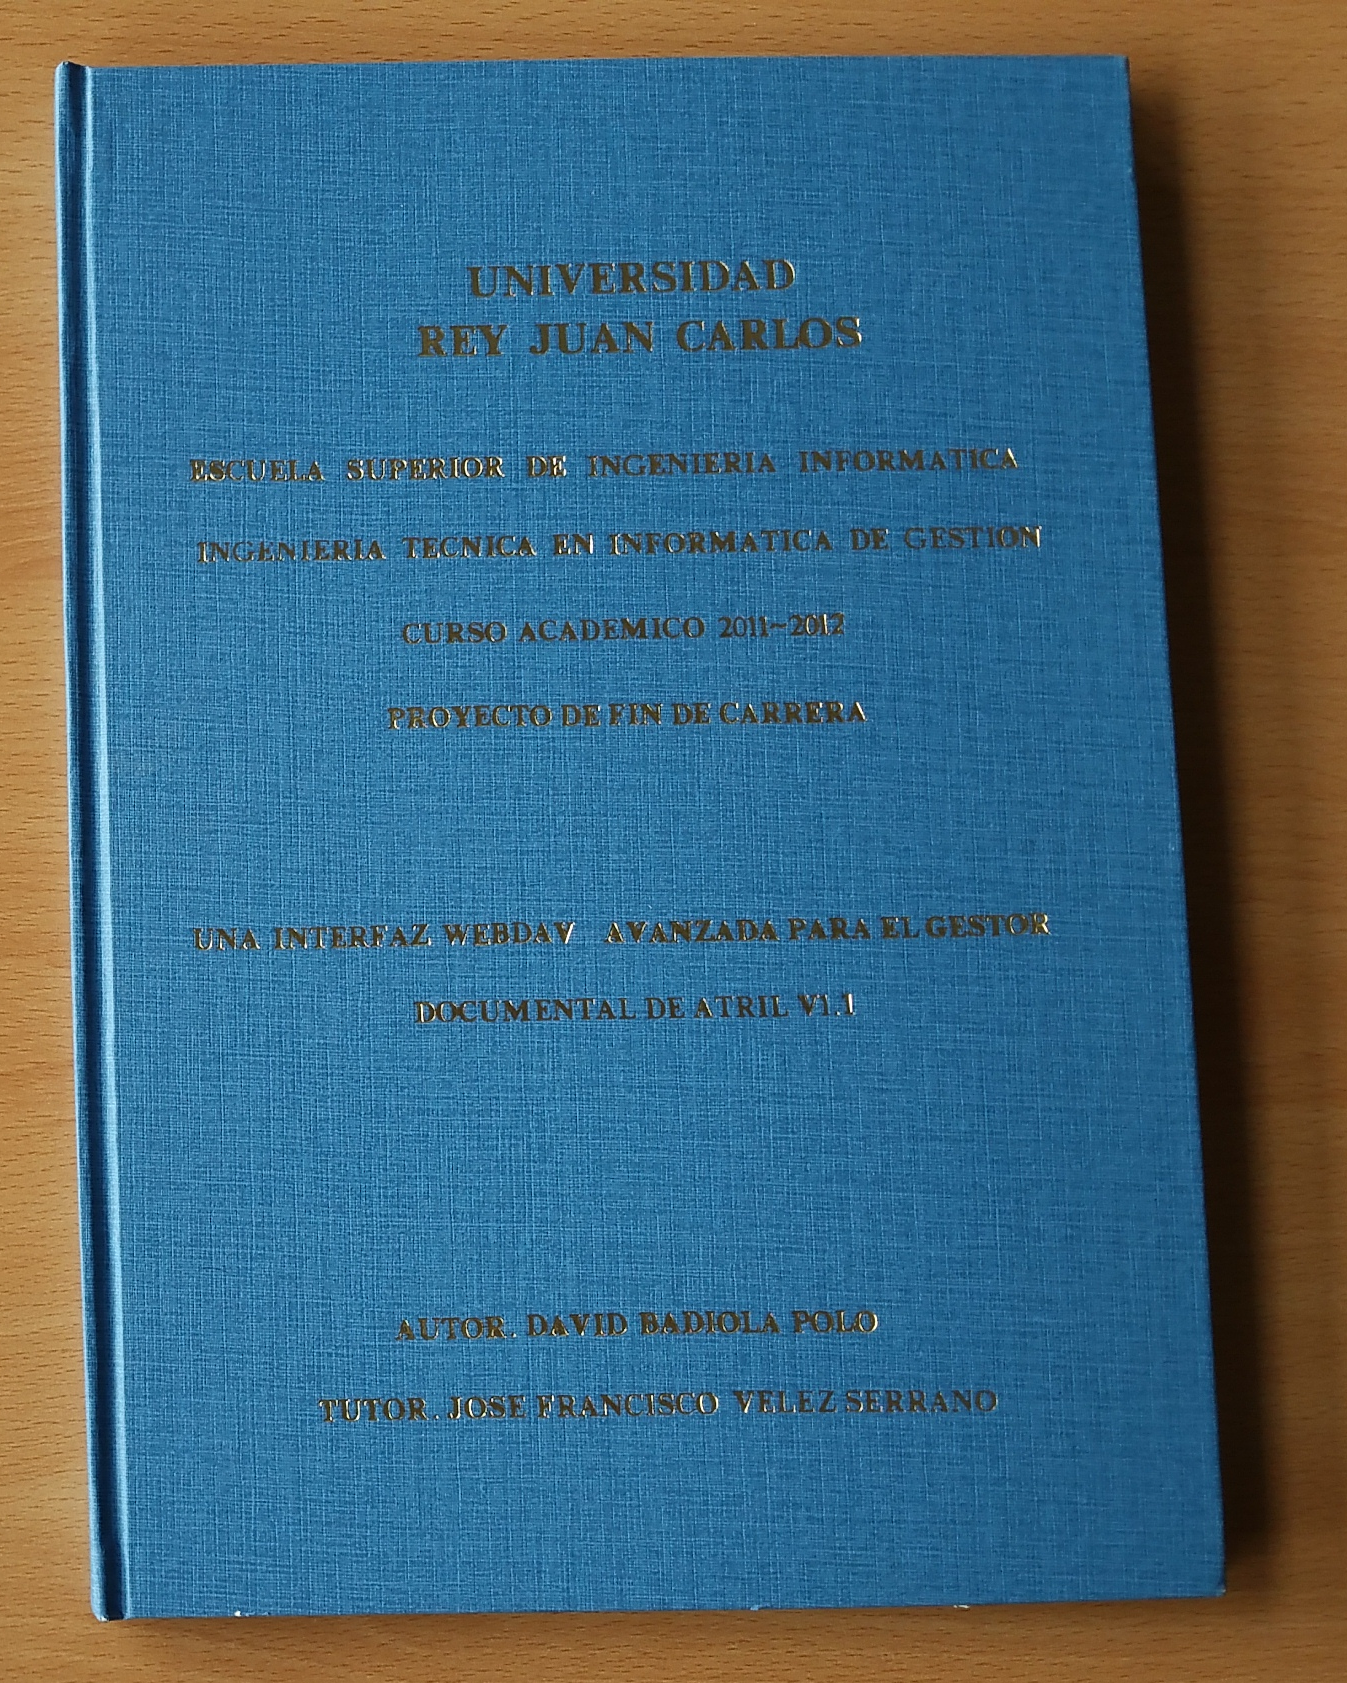
\includegraphics[height=7cm]{Figs/EncuadernacionCara}\hspace{2cm}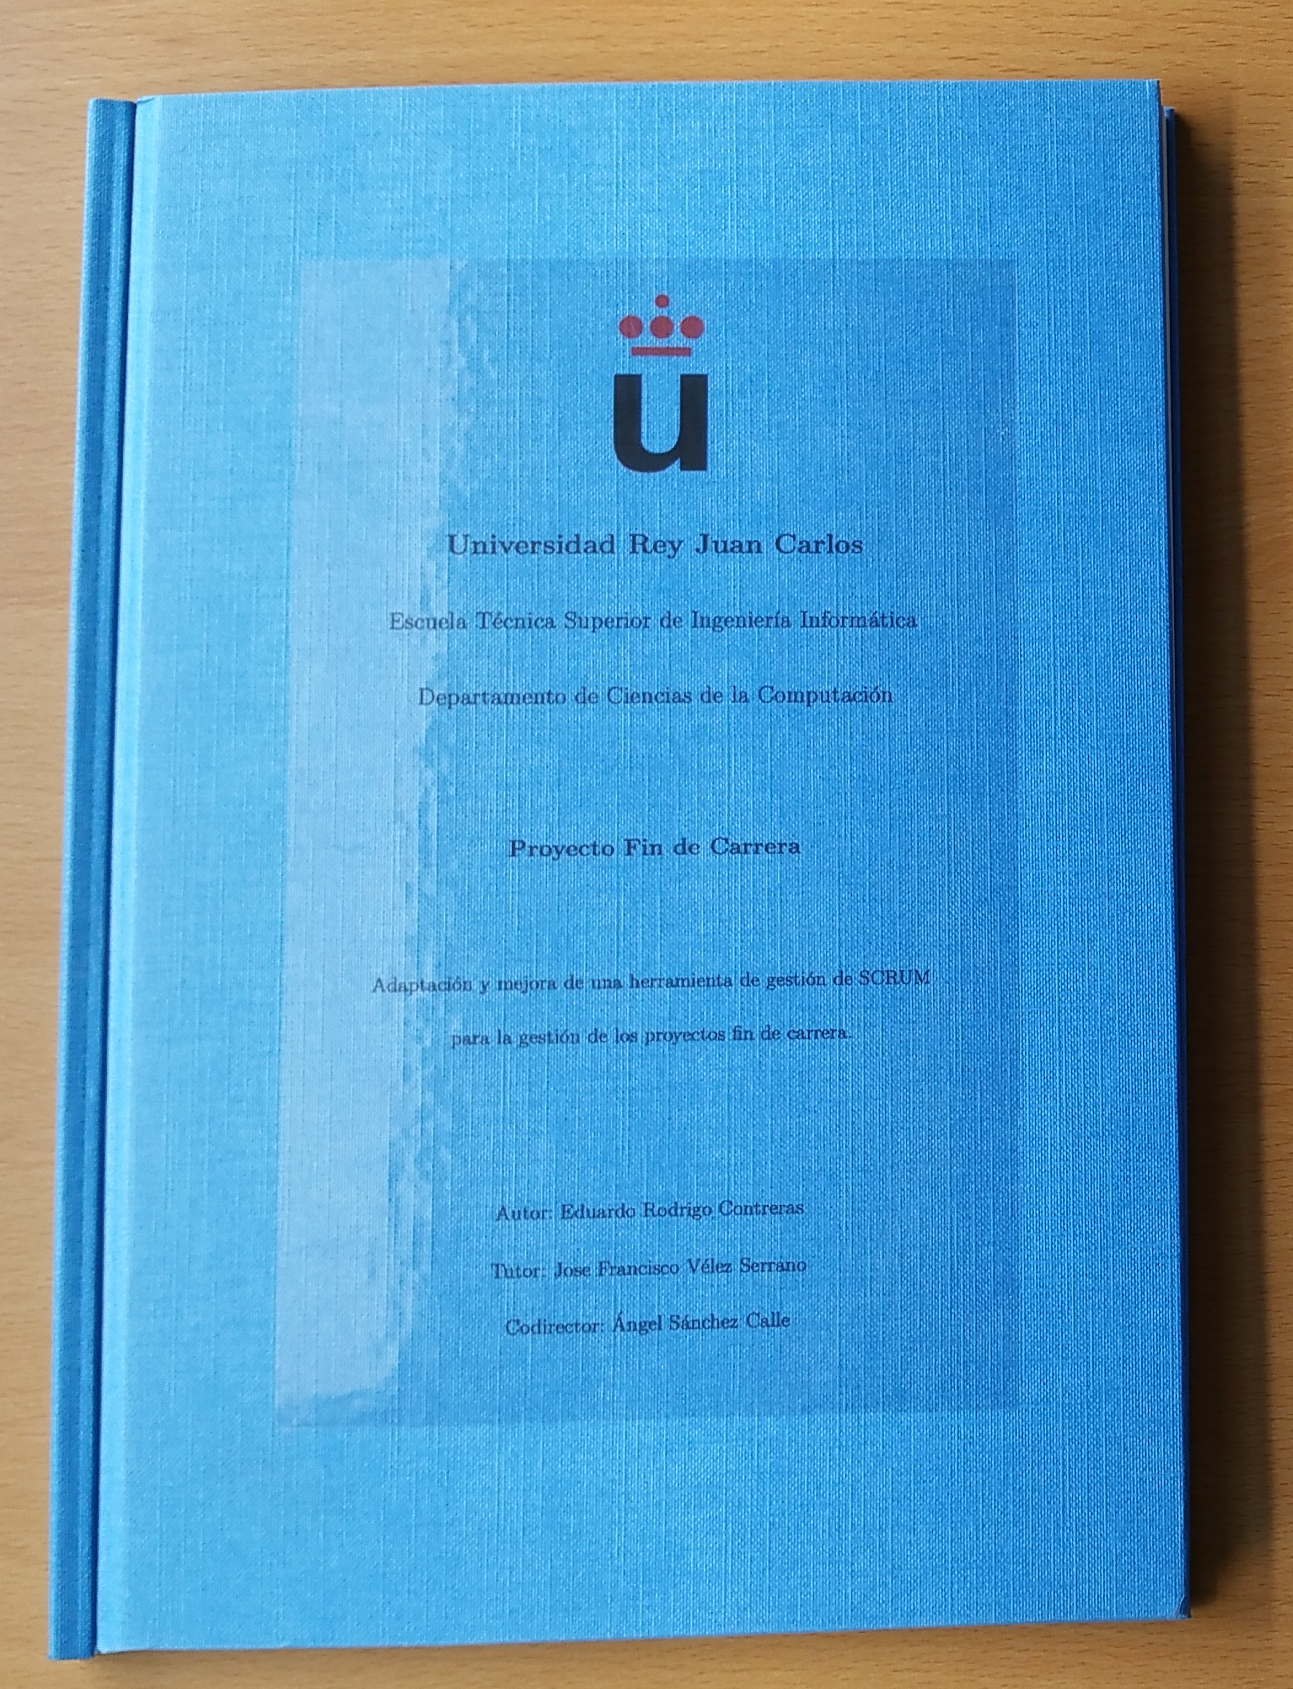
\includegraphics[height=7cm]{Figs/EncuadernacionBarata}
            \par\end{centering}
        \begin{centering}
        (a)\hspace{7cm}(b)
        \par\end{centering}
        \caption[Ejemplos de encuadernaciones para la memoria.]{Ejemplos de encuadernaciones para la memoria. En (a) una encuadernación
        de más calidad aunque más cara. En (b) una encuadernación más barata
        y suficiente.\label{fig:Ejemplos-de-encuardenaciones}}
    \end{figure}

    \subsection{Terminología y concepto de la contabilidad descentralizada}

    \subsection{Beneficios de Blockchain en la contabilidad financiera }


    \chapter{Idea de negocio}

    Las memorias de los TFT suelen ser documentos académicos, formales,
    muy explicativos, autocontenidos en cuanto a lo que ha desarrollado
    el alumno, con muchas referencias y sin afirmaciones gratuitas. Además,
    debe cuidarse su redacción, su ortografía y su ortotipografía. En
    las siguientes secciones se desarrollan estas ideas.

    \section{Desarrollo de modelo de negocio}

    El documento se compondrá de capítulos\index{capítulos} y secciones\index{secciones}
    anidadas dentro de los capítulos. Cada título de sección o de subsección
    debe ir seguido de uno o más párrafos que expliquen, al menos, qué
    se va a contar en dicho capítulo, sección o subsección. No deben aparecer
    nunca títulos aislados o seguidos de otros títulos.

    Los párrafos\index{párrafos} de texto serán los verdaderos responsables
    de explicar lo que se ha hecho en el TFT. Suele ser una buena idea
    diseñar un esquema de lo que se desea contar en cada capítulo, sección
    y párrafo.

    Al escribir los párrafos, en general se recomienda un estilo impersonal,
    evitando el ``yo'' o el ``nosotros''. Así, normalmente se utilizarán
    frases en pasivo y pasivo reflejo. Es importante el uso del corrector
    ortográfico, pero también debe revisarse con atención las palabras
    que siendo correctas (porque están en el diccionario) no se emplean
    de manera adecuada (por ejemplo poner ``Haber'' en vez de ``A ver'',
    ``a'' en lugar de ``ha'', ``tilde'' en lugar de ``tildé'',
    ``qué'' en lugar de ``que'', o cualquier tilde diacrítica).

    También es recomendable utilizar frases cortas, ya que en ellas las
    ideas se transmiten con más simplicidad y es más difícil cometer errores.
    Por ejemplo, los siguiente dos puntos explican lo mismo:
    \begin{itemize}
        \item Muchos autores ({[}5{]},{[}18{]},{[}33{]}) utilizan la medida del
        TF-IDF por ser altamente representativa de la importancia que tiene
        cada término dentro de un corpus, habiéndose convertido en un referente
        en el ámbito de la minería de textos.
        \item El TF-IDF muestra la relevancia de cada termino en un corpus. Esta
        medida es habitual en el campo de la minería de textos, siendo usada
        por autores como {[}5{]}, {[}18{]} y {[}33{]}.
    \end{itemize}
    Para empezar, el primer párrafo incurre en varias inexactitudes:
    \begin{itemize}
        \item Solo se citan tres autores, y se dice que son muchos autores. Desde
        cuando tres son muchos.
        \item El primer punto dice que el TF-IDF ``es un referente en el ámbito
        de la minería de datos''. ¿Quién lo dice o qué estudio se ha realizado
        para asegurar esto?.
    \end{itemize}
    Además, aunque podría parecernos que el primer párrafo tiene mejor
    estilo literario, la realidad es que el segundo párrafo expone las
    dos ideas que se quiere transmitir con mayor claridad. Estas dos ideas
    son: qué hace el TF-IDF y cómo de común es su uso.

    \section{Potencial del modelo de negocio}

    Todo lo que se deba contar respecto al TFT debe estar en la memoria.
    La memoria no debe dejar dudas respecto a lo qué se ha hecho, cómo
    se ha hecho o por qué se ha hecho. Para ello lo mejor es seguir todo
    lo que se ha apuntado en el cuaderno de trabajo (que se habrá utilizado
    durante el desarrollo del TFT), de manera que no quede nada sin explicar.

    Parte de esta característica de autocontenido consiste en que en que
    cada vez que se utilice un término técnico se explique. También, en
    el caso de siglas\index{siglas} y acrónimos\index{acrónimos} siempre
    se deben introducir explicándolos antes de usarlos.

    En cualquier caso se recomienda seguir un discurso ordenado, que describa
    paso a paso desde el principio todo lo que se ha ido haciendo hasta
    concluir el TFT.

    \section{Transparencia, seguridad e inmutabilidad de los datos}

    Todo lo que se dice en una memoria de TFT debe ser verdad, pero además
    debe citarse la fuente o describirse por qué se sabe que es verdad.
    Así, si se obtiene una conclusión de un desarrollo o de un experimento,
    dicha conclusión será verdad porque está explicada en la propia memoria.
    Pero si se afirma algo que no se deriva de los experimentos de la
    memoria se debe citar mediante una referencia quién afirma dicha verdad.

    Por ejemplo, si se dijese que los TFT siempre suelen estar bien redactados
    hay dos opciones. O bien la afirmación se acompaña de una referencia
    a algún estudio que lo demuestre, o bien se realiza un estudio para
    poder afirmarlo. En este último caso habría que revisar una muestra
    de TTFFGG y realizar un estudio estadístico sobre su redacción.

    Como siempre, estas reglas deben tomarse con mesura. En una memoria
    no hay que demostrar que dos y dos suman cuatro, ya que este es un
    conocimiento común y ampliamente aceptado.

    \section{Garantía de la imagen fiel de las empresas}

    La memoria de un Trabajo Fin de Grado es una obra literaria y como
    a tal se le exige unos requisitos mínimos que no hagan desagradable
    su lectura. En los siguientes párrafos se mencionan algunos aspectos
    que deben cuidarse.

    \section{Validación de negocio y modelo canvas}

    En primer lugar hay que diferenciar al narrador del autor y del escritor.

    El autor de un libro es el que piensa lo que hay que escribir, el
    escritor es el que lo escribe y el narrador es el que relata el documento.

    Normalmente, el autor y el escritor suelen ser la misma persona, pero
    en ocasiones no es así. Por ejemplo, Jorge Luis Borges continuó escribiendo
    aún cuando se quedó prácticamente ciego gracias a su secretaria y
    luego esposa, María Kodama y a varios ayudantes enviados por sus editoriales.
    Normalmente, en los TFT el autor y el escritor son la misma persona
    \cite{Leo2014}.

    Respecto al narrador se puede optar por usar diferentes estilos. Así,
    la memoria de un TFT se suele escribir en impersonal, en primera persona
    del singular o en primera persona del plural. Los siguientes párrafos
    ilustran cada caso:
    \begin{itemize}
        \item Ejemplo de impersonal: En esta memoria \emph{se describen} los procesos
        que han permitido\emph{ }a un alumno obtener una alta nota en la memoria
        del TFT.
        \item Ejemplo de primera persona del singular: En esta memoria \emph{describo}
        los procesos que me han permitido obtener una alta nota en la memoria
        del TFT.
        \item Ejemplo de primera persona del plural: En esta memoria \emph{describimos}
        los procesos que han permitido al alumno obtener una alta nota en
        la memoria del TFT.
    \end{itemize}
    El estilo preferido en un trabajo científico suele ser el impersonal,
    ya que suele fomentar la no implicación personal del autor en la evaluación
    de los hechos científicos presentados. Aún así, la elección del narrador
    es una decisión personal.

    \chapter{Conclusiones}

    En este capítulo se resumen los objetivos conseguidos, se presentan
    las conclusiones y las posibles continuaciones de este trabajo.

    \section{Objetivos cumplidos}

    El presente documento cumple los objetivos descritos en la introducción
    respecto a servir de guía para la confección de las memorias de los
    TFT.

    En concreto, el documento desarrollado cumple los objetivos específicos
    planteados. Así:
    \begin{itemize}
        \item Orienta al alumno y al profesor respecto al índice del TFT en las
        diferentes titulaciones.
        \item Ofrece al alumno una plantilla para documentos de tipo de TFT. Dicha
        plantilla está disponible para el procesador Lyx y para el procesador
        Writer de LibreOffice.
        \item Detalla los elementos documentales que debe manejar una memoria de
        TFT (índices, tablas de contenidos, notas a pie de página...).
        \item Aconseja al alumno en cuanto al estilo literario.
        \item Explica al alumno cómo utilizar el procesador de textos para confeccionar
        este tipo de documentos.
        \item Propone una guía para la presentación del TFT.
    \end{itemize}

    \section{Futuras mejoras}

    Entre los futuros trabajos de este documento se plantea la ampliación
    de esta guía a más tipos de grados.

    \appendix

    \chapter{Anexo}

    Este anexo describe el proceso de instalación de Lyx en diferentes
    sistemas operativos.

    \section*{\cleardoublepage}

    \printbibliography[heading=bibintoc]

    \printindex
\end{document}
